\documentclass[a4paper,12pt]{article}
\usepackage[a4paper,top=1.3cm,bottom=2cm,left=1.5cm,right=1.5cm,marginparwidth=0.75cm]{geometry}

% Пакеты
\usepackage{mathtext}
\usepackage{setspace}
\usepackage{tabularx}
\usepackage{cmap}
\usepackage{longtable}
\usepackage{icomma}
\usepackage{euscript}
\usepackage{float} % Убедитесь, что пакет float загружен
\usepackage{cutwin}
\usepackage{mathrsfs}
\usepackage{adjustbox}
\usepackage{dashbox}
\usepackage[normalem]{ulem}
\usepackage[T2A]{fontenc}
\usepackage[utf8]{inputenc} %! закрепляет кодировку utf8
\usepackage[english,russian]{babel} %! подключает русский и английский
%математические шрифты:
\usepackage{amsmath,amsfonts,amssymb,amsthm,mathrsfs,mathtools}
\usepackage[colorlinks, linkcolor = purple]{hyperref} %! оглавление для панели навигации по PDF-документу + гиперссылки
\usepackage{xcolor} %! добавляет цвета
\usepackage{enumitem} %! задание макета перечня.
\usepackage{xpatch} %? работа с renewcommand и макросами
\usepackage{cancel} % зачёкивания текста (!!!) для slash-нотации использовать \usepackage{slashed}!!
\usepackage{upgreek} % заглавные греческие буквы
\usepackage{lipsum} %? для вставки кучи текста при форматировании
\usepackage[version=4]{mhchem} % химические формулы
\usepackage{multirow} % объединение строк в матрицах
\usepackage{stackengine} % stack символов
\usepackage{tikz} %! рисунки
\usetikzlibrary{positioning} %? библиотека для тикза
\usepackage{titletoc} %! форматирование содержания и заголовков
\usepackage{titlesec} %! форматирование содержания и заголовков
\usepackage{wrapfig} % обтекание таблиц и рисунков
\usepackage{chngcntr} %! для setcounter
\usepackage{fancyhdr} %! для колонтитулов
\usepackage{makecell} %? матрицы с разными выравниваниями и т.п
\usepackage{indentfirst} % добавить indent перед первым
\usepackage{tocloft} %? изменение названий глав и разделов
\usepackage{soul} % типографические примочки, типо зачёркивания и подчёркивания
\usepackage[stable]{footmisc} %? продвинутые сноски
\usepackage{subfig} % несколько картинок рядом

\mathtoolsset{showonlyrefs=true}

%Обозначения теорем и т.п
\theoremstyle{definition}
\newtheorem*{definition}{Определение}
\newtheorem{statement}{Предложение}[section]
\newtheorem{lemma}{Лемма}[section]
\newtheorem{theorem}{Теорема}[section]
\newtheorem*{theoremn}{Теорема}
\newtheorem*{corollary}{Следствие}
\newtheorem*{example}{Пример}
\newtheorem*{note}{Замечание}
\newtheorem*{problem}{Задача}

%Шарабара для содержания и внешнего вида нумерации
\counterwithout{footnote}{section}\DeclareRobustCommand{\divby}{%
\mathrel{\text{\vbox{\baselineskip.65ex\lineskiplimit0pt\hbox{.}\hbox{.}\hbox{.}}}}%
}

%Разные операторы и символы
\newcommand{\dotpr}[2]{\bra{#1}\ket{#2}}
\let\AA\relax
\let\emptyset\varnothing
\DeclareMathOperator*{\esssup}{ess sup}
\DeclareMathOperator*{\ord}{ord}
\DeclareMathOperator*{\supp}{supp}
\DeclareMathOperator*{\pr}{pr}
\DeclareMathOperator*{\Ker}{Ker}
\DeclareMathOperator*{\Vol}{Vol}
\DeclareMathOperator*{\rg}{rk}
\DeclareMathOperator*{\Ima}{Im}
\DeclareMathOperator*{\Alt}{Alt}
\DeclareMathOperator*{\Sym}{Sym}
\newcommand{\eqdef}{\stackrel{\text{\tiny{def}}}{=}}
\newcommand{\pp}{\partial}
\newcommand{\AA}{\mathcal{A}}
\newcommand{\BB}{\mathcal{B}}
\newcommand{\MM}{\mathbb{M}}
\newcommand{\NN}{\mathbb{N}}
\newcommand{\ZZ}{\mathbb{Z}}
\newcommand{\QQ}{\mathbb{Q}}
\newcommand{\RR}{\mathbb{R}}
\newcommand{\CC}{\mathbb{C}}
\newcommand{\FFF}{\mathbb{F}}
\newcommand{\DD}{\mathcal{D}}
\newcommand{\FF}{\mathcal{F}}
\newcommand{\sS}{\mathcal{S}}
\newcommand*\circled[1]{\tikz[baseline=(char.base)]{

ode[shape=circle,draw,inner sep=2pt] (char) {#1};}}

\title{СПЕКТРАЛЬНЫЙ АНАЛИЗ ЭЛЕКТРИЧЕСКИХ СИГНАЛОВ (3.6.1)}
\author{Пазов Тенгиз\\
Симухин Егор}
\date{\today}

\begin{document}

\maketitle
\section{Аннотация}
\indent
\indent \textbf{Цель работы:} изучить спектры сигналов различной формы и влияние параметров сигнала
на вид соответствующих спектров; проверить справедливость соотношений неопределённостей; познакомиться с работой спектральных фильтров на примере RC-цепочки

\indent \textbf{В работе используются:} генератор сигналов произвольной формы, цифровой осциллограф с функцией быстрого преобразования Фурье или цифровой USB-осциллограф, подключённый к персональному компьютеру.

\section{Теоретическое введение}

\subsection*{Разложение сложных сигналов на периодические колебания}
Представление периодического сигнала в виде суммы гармонических сигналов называется разложением в ряд Фурье.

Пусть заданная функция $f(t)$ периодически повторяется с частотой $\Omega_{1}=\dfrac{2\pi}{T},$ где $T$ - период повторения. Ее разложение в ряд Фурье имеет вид
\begin{equation}
f(t)=\dfrac{a_{0}}{2}+ \sum\limits_{n=1}^\infty [a_{n}\cos(n \Omega_{1}t)+b_{n}\sin(n \Omega_{1} t) ]
\label{eq1}
\end{equation}
Здесь $\dfrac{a_{0}}{2}$ - среднее значение функции $f(t)$,

\begin{equation}
a_{n}=\dfrac{2}{T}\int\limits_{t_{1}}^{t_{1}+T}f(t)\cos(n \Omega_{1} t)dt,
\label{eq2}
\end{equation}
\begin{equation}
b_{n}=\dfrac{2}{T}\int\limits_{t_{1}}^{t_{1}+T}f(t)\sin(n \Omega_{1} t)dt.
\label{eq3}
\end{equation}

Рассмотрим периодические функции, которые исследуются в нашей
работе.

\begin{enumerate}

\item \textbf{Периодическая последовательность прямоугольных импульсов} (рис. 1) с амплитудой $V_{0}$, длительностью $\tau$, частотой повторения $\Omega_{1}=\dfrac{2\pi}{T},$ где $T$ - период повторения импульсов. Найдем коэффициенты разложения ряда Фурье:

$$\dfrac{a_{0}}{2}=V_{0}\dfrac{\tau}{T},$$

\begin{equation}
a_{n}=\dfrac{2}{T}\int\limits_{-\frac{\tau}{2}}^{\frac{\tau}{2}}V_{0}\cos(n \Omega_{1} t)dt=2V_{0}\dfrac{\tau}{T}\dfrac{\sin(n \Omega_{1} \frac{\tau}{2})}{n\Omega_{1}\frac{\tau}{2}} \sim \dfrac{\sin x}{x}.
\label{eq4}
\end{equation}

Поскольку наша функция четная, все коэффициенты синусоидальных гармоник $b_{n}=0$. Спектр $a_{n}$ последовательности прямоугольных импульсов представлен на рис. 2 (изображен случай, когда $T$ кратно $\tau$).

\begin{figure}[H] % Изменение на [H]
\begin{minipage}[h]{0.5\linewidth}
\center{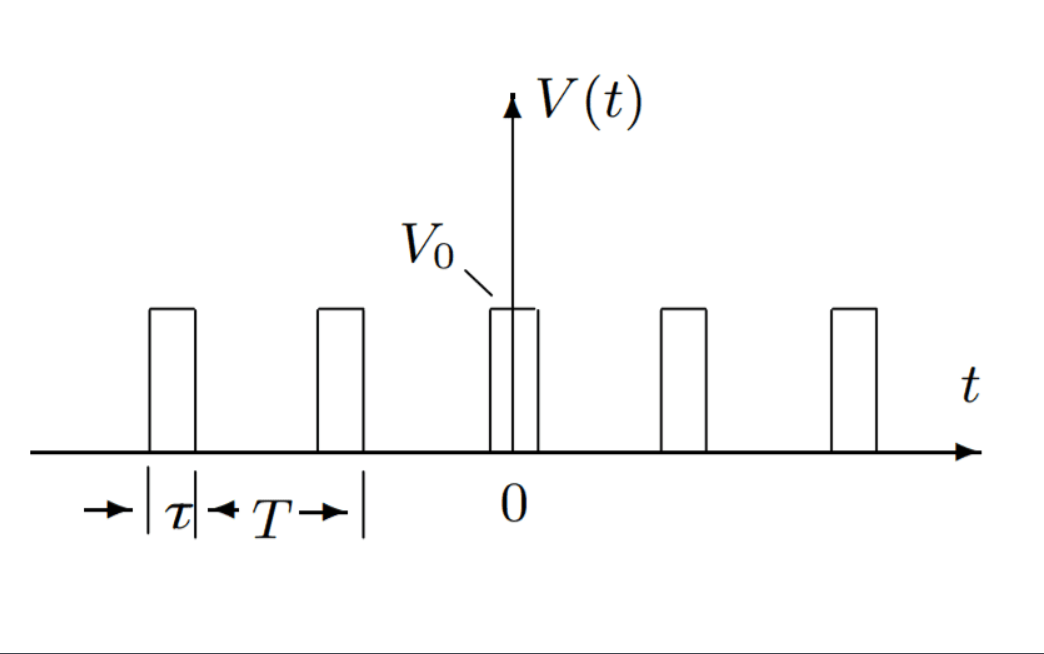
\includegraphics[width=0.9\linewidth]{Снимок экрана 2024-12-14 012419.png}}
\caption{Прямоугольные импульсы}
\end{minipage}
\begin{minipage}[h]{0.5\linewidth}
\center{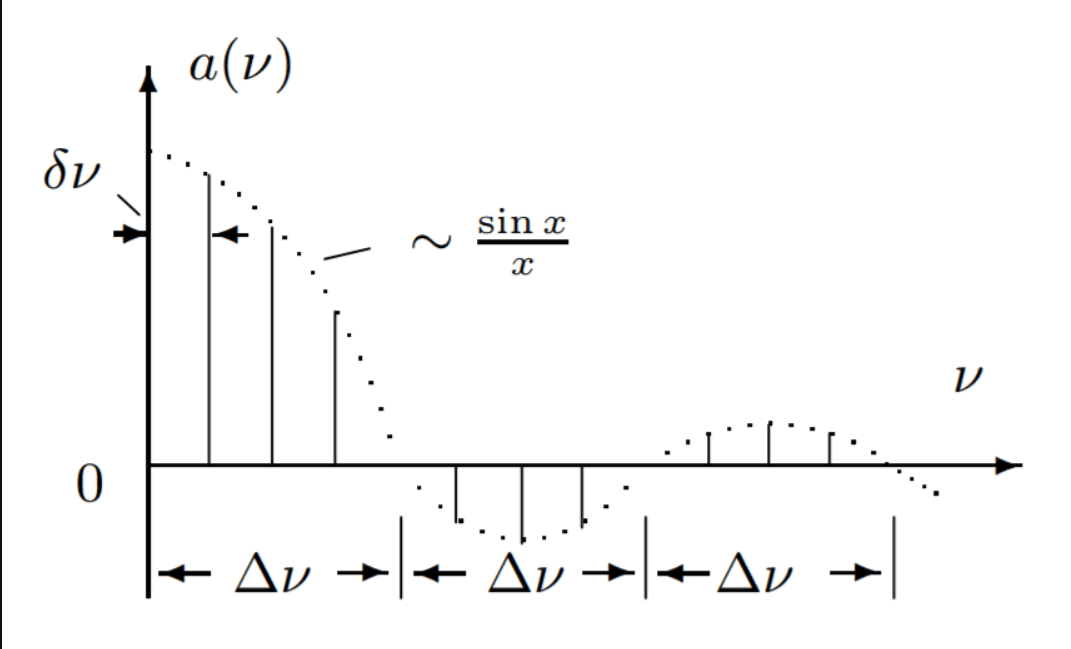
\includegraphics[width=0.9\linewidth]{Снимок экрана 2024-12-14 012503.png}}
\caption{Спектр последовательности прямоугольных импульсов}
\end{minipage}
\end{figure}

Назовем \textit{шириной спектра} $\Delta \omega$ расстояние от главного максимума ($\omega =0$) до первого нуля огибающей, возникающего при $n=\dfrac{2\pi}{\tau \Omega_{1}}$. При этом

$$\Delta \omega \tau \backsimeq 2 \pi $$

или

\begin{equation}\label{neopr}
\Delta \nu \Delta t \backsimeq 1
\end{equation}

Полученное соотношение взаимной связи интервалов $\Delta \nu$ и $\Delta t$ является
частным случаем соотношения неопределенности в квантовой механике.

\item \textbf{Периодическая последовательность цугов} гармонического колебания $V_{0}\cos(\omega_{0}t)$ с длительностью цуга $\tau$ и периодом повторения $T$ (рис. 3).

Функция $f(t)$ снова является четной относительно $t=0$. Коэффициент при $n$-й гармонике равен
\begin{equation}
a_{n}=\dfrac{2}{T}\int\limits_{-\frac{\tau}{2}}^{\frac{\tau}{2}}V_{0}\cos(\omega_{0}t)\cos(n \Omega_{1}
t)dt=V_{0}\dfrac{\tau}{T} \bigg(\dfrac{\sin[(\omega_{0}-n\Omega_{1})\frac{\tau}{2}]}{(\omega_{0}-n\Omega_{1})\frac{\tau}{2}}+\dfrac{\sin[(\omega_{0}+n\Omega_{1})\frac{\tau}{2}]}{(\omega_{0}+n\Omega_{1})\frac{\tau}{2}} \bigg)
\label{eq6}
\end{equation}

Зависимость для случая, когда $\frac{T}{\tau}$ равно целому числу, представлена на рис. 4. Сравнивая спектр последовательности прямоугольных импульсов и цугов мы видим, что они аналогичны, но их максимумы сдвинуты по частоте на величину $\omega_{0}$.

\begin{figure}[H] % Изменение на [H]
\begin{minipage}[h]{0.5\linewidth}
\center{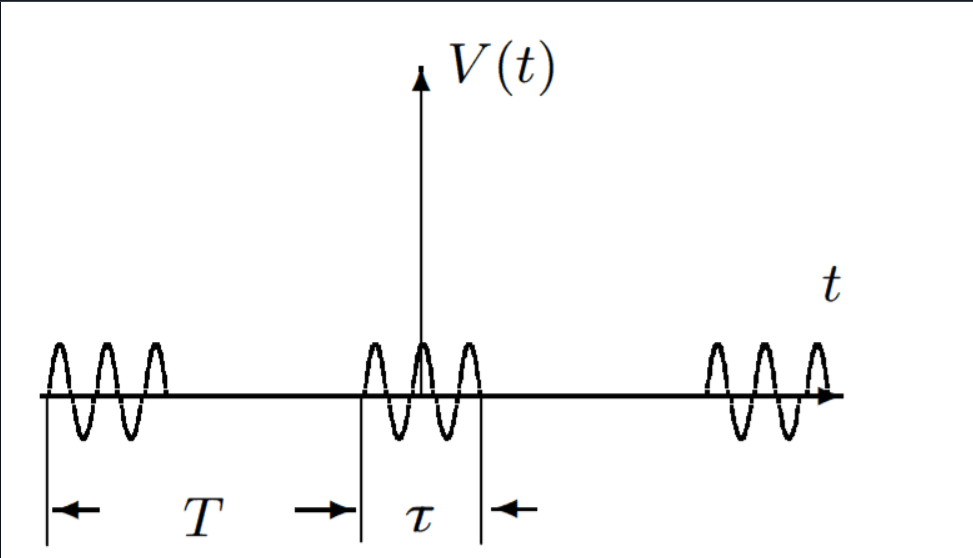
\includegraphics[width=0.9\linewidth]{Снимок экрана 2024-12-14 012703.png}}
\caption{Последовательность цугов}
\end{minipage}
\begin{minipage}[h]{0.5\linewidth}
\center{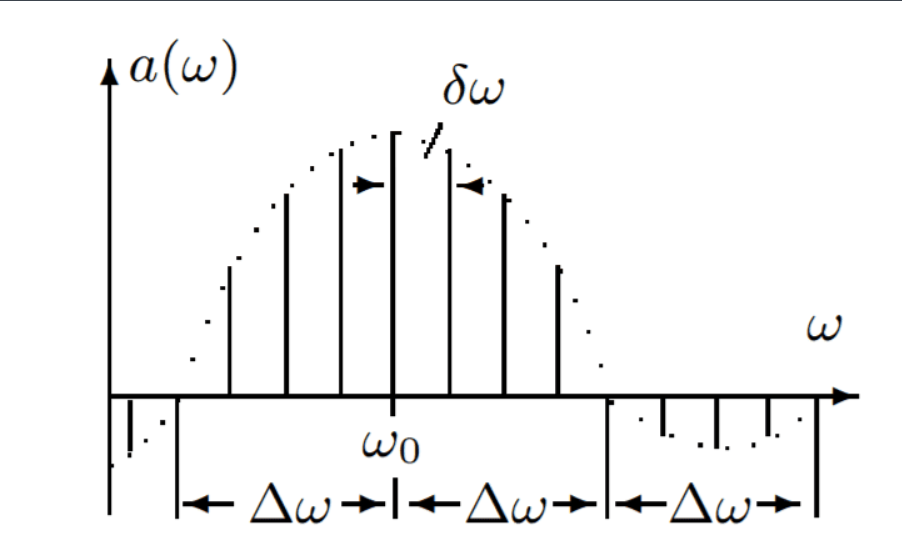
\includegraphics[width=0.9\linewidth]{Снимок экрана 2024-12-14 012720.png}}
\caption{Спектр последовательности цугов}
\end{minipage}
\end{figure}

\item \textbf{Амплитудно-модулированные колебания.} Рассмотрим гармонические колебания высокой частоты $\omega_{0}$ , амплитуда которых медленно меняется по гармоническому закону с частотой $\Omega$ ($\Omega \ll \omega_{0})$) (рис. 5):
\begin{equation}
f(t)=A_{0}[1+m\cos\Omega t]\cos \omega_{0}t
\label{eq7}
\end{equation}

Коэффициент $m$ называют \textbf{глубиной модуляции}. При $m<1$ амплитуда колебаний меняется от минимальной $A_{min}=A_{0}(1-m)$ до максимальной $A_{max}=A_{0}(1+m).$ Глубина модуляции может быть представлена в виде

\begin{equation}\label{m}
m=\dfrac{A_{max}-A_{min}}{A_{max}+A_{min}}
\end{equation}

Простым тригонометрическим преобразованием можно найти спектр амплитудно - модулированных колебаний:
\\
\begin{equation}\label{a}
f(t)=A_{0}\cos(\omega_{0} t)+\dfrac{A_{0}m}{2}\cos(\omega_{0}+\Omega)t+\dfrac{A_{0}m}{2}\cos(\omega_{0}-\Omega)t.
\end{equation}

\begin{figure}[H] % Изменение на [H]
\begin{minipage}[h]{0.5\linewidth}
\center{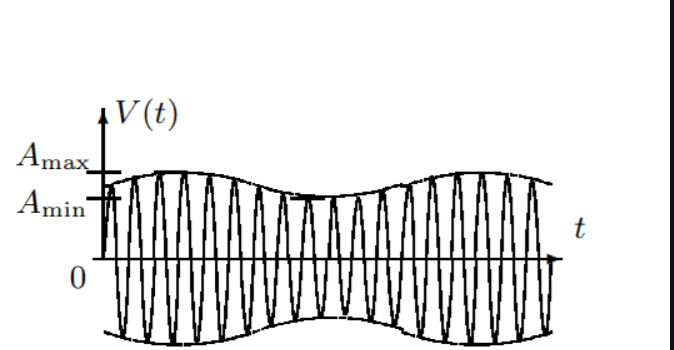
\includegraphics[width=0.9\linewidth]{Снимок экрана 2024-12-14 012751.png}}
\caption{Модулированные гармонические колебания}
\end{minipage}
\begin{minipage}[h]{0.5\linewidth}
\center{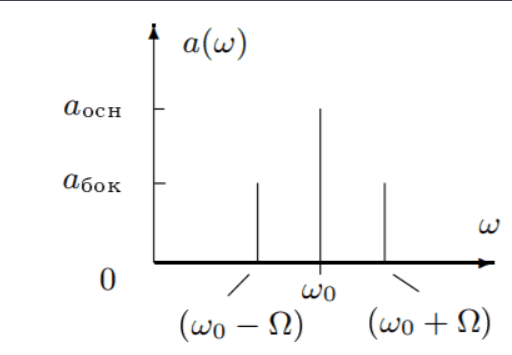
\includegraphics[width=0.9\linewidth]{Снимок экрана 2024-12-14 012824.png}}
\caption{Спектр модулированных гармонических колебаний}
\end{minipage}
\end{figure}

Спектр таких колебаний содержит три составляющих основную
компоненту и две боковых (рис. 6). Первое слагаемое в правой части представляет собой исходное немодулированное колебание
с основной (несущей) частотой $\omega_{0}$ и амплитудой $a_{осн} = A_{0}$ . Второе и третье слагаемые соответствуют новым гармоническим колебаниям с частотами $\omega_{0} + \Omega$ и $\omega_{0} - \Omega$. Амплитуды этих двух колебаний одинаковы и составляют $\dfrac{m}{2}$ от амплитуды немодулированного колебания:
$a_{бок} = \dfrac{A_{0}m}{2}$. Начальные фазы всех трех колебаний одинаковы.
\end{enumerate}

\section{Ход работы}

\subsection*{А. Исследование спектра периодической последовательности
прямоугольных импульсов и проверка соотношений неопределённости}

\begin{enumerate}

\item [\textbf{1.}] Настраиваем генератор на прямоугольные импульсы с частотой повторения $\nu_\text{повт}$ = 1 кГц (период $T$ = 1 мс) и
длительностью импульса $\tau$ = $T$/20 = 50 мкс.

\item [\textbf{2.}] Получаем на экране спектр (Преобразование Фурье) сигнала.

\textbf{a.} Изменяем $\nu_\text{повт}$ при фиксированном $\tau$ = 50 мкс и получаем:

\begin{figure}[H] % Изменение на [H]
\begin{minipage}[h]{0.47\linewidth}
\center{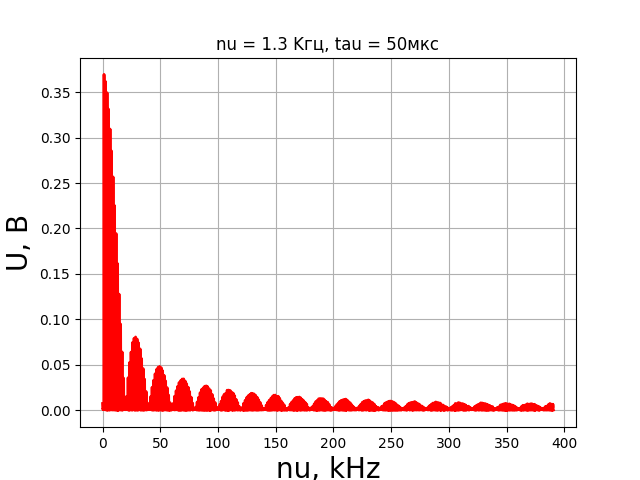
\includegraphics[width=1\linewidth]{tau=50nu=1.3kHz.png}} \\$\nu_\text{повт}$ = 1 кГц
\end{minipage}
\hfill
\begin{minipage}[h]{0.47\linewidth}
\center{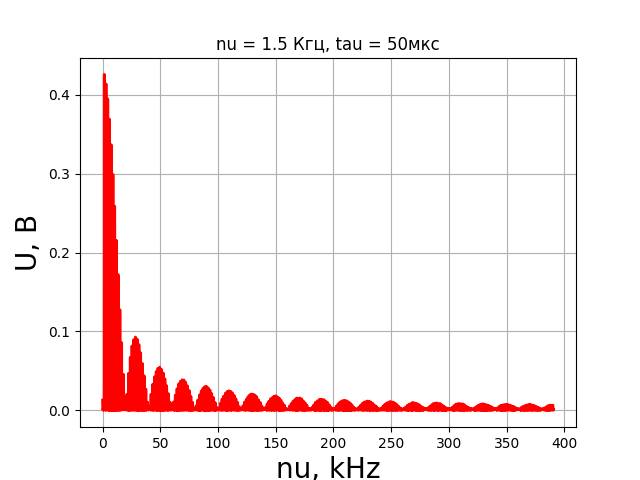
\includegraphics[width=1\linewidth]{tau=50nu=1.5kHz.png}} \\$\nu_\text{повт}$ = 2 кГц
\end{minipage}
\vfill
\begin{minipage}[h]{0.47\linewidth}
\center{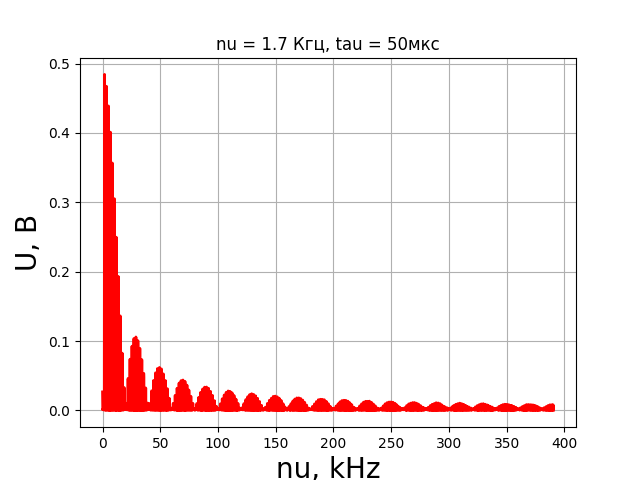
\includegraphics[width=1\linewidth]{tau=50nu=1.7kHz.png}} $\nu_\text{повт}$ = 5 кГц \\
\end{minipage}
\hfill
\begin{minipage}[h]{0.47\linewidth}
\center{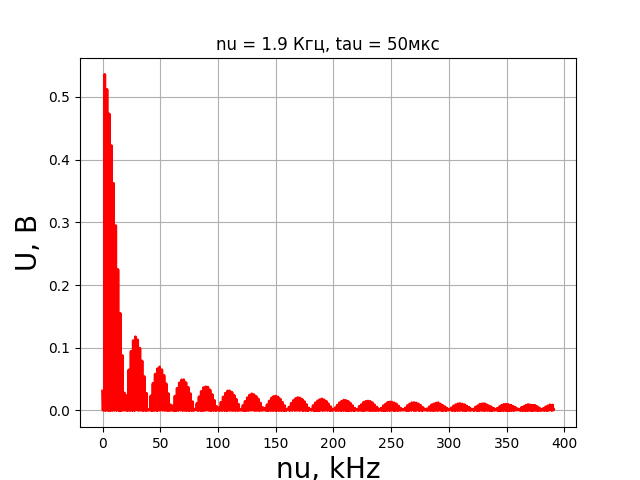
\includegraphics[width=1\linewidth]{tau=50nu=1.9kHz.png}} $\nu_\text{повт}$ = 10 кГц \\
\end{minipage}
\caption{}
\label{ris:experimentalcorrelationsignals}
\end{figure}

Как видно из графиков, при увеличении частоты повторения сигнала увеличивается
расстояние между компонентами спектра.


\textbf{б.} Изменяем $\tau$ при фиксированном $\nu_\text{повт}$ = 1 кГц и получаем:

\begin{figure}[h!] 
\centering % Центрируем всю фигуру
\begin{minipage}[t]{0.45\linewidth} % Изменил ширину на 0.45
    \centering
    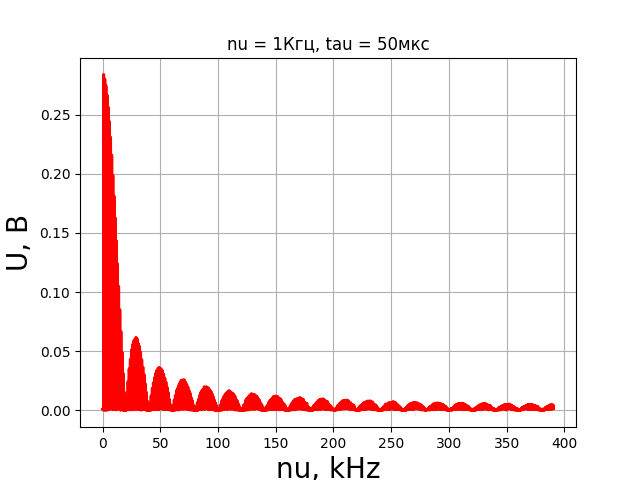
\includegraphics[width=\linewidth]{nu=1kHztau=50mks.png} 
    \caption*{$\tau$ = 50 мкс} % Используем caption* для подзаголовка
\end{minipage}
\hfill
\begin{minipage}[t]{0.45\linewidth} % Изменил ширину на 0.45
    \centering
    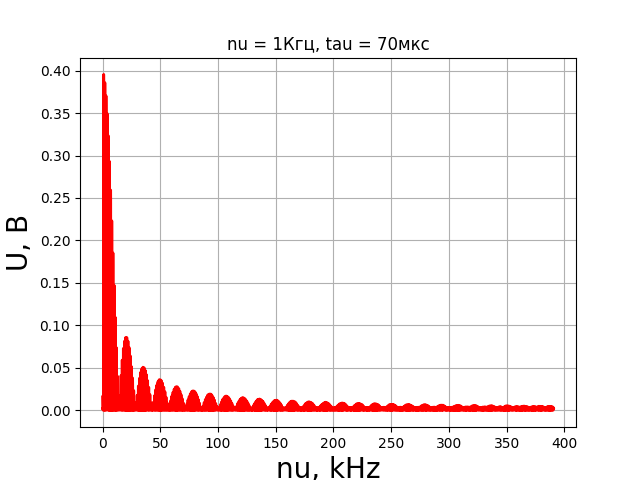
\includegraphics[width=\linewidth]{nu=1kHztau=70mks.png} 
    \caption*{$\tau$ = 70 мкс}
\end{minipage}

\vspace{0.5cm} % Добавляем отступ между строками графиков
\begin{minipage}[t]{0.45\linewidth} % Изменил ширину на 0.45
    \centering
    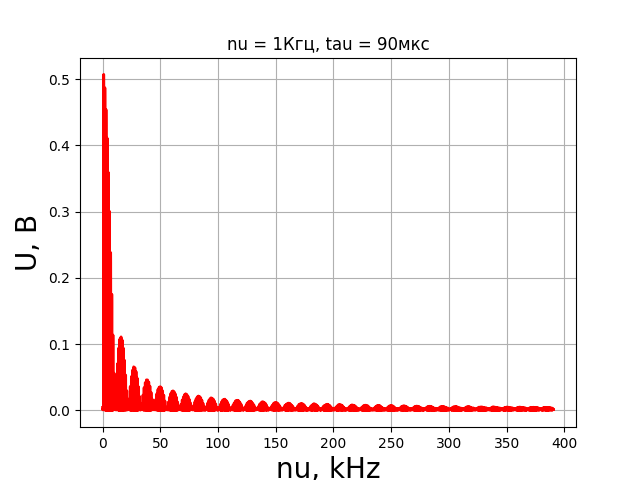
\includegraphics[width=\linewidth]{nu=1kHztau=90mks.png} 
    \caption*{$\tau$ = 90 мкс}
\end{minipage}
\hfill
\begin{minipage}[t]{0.45\linewidth} % Изменил ширину на 0.45
    \centering
    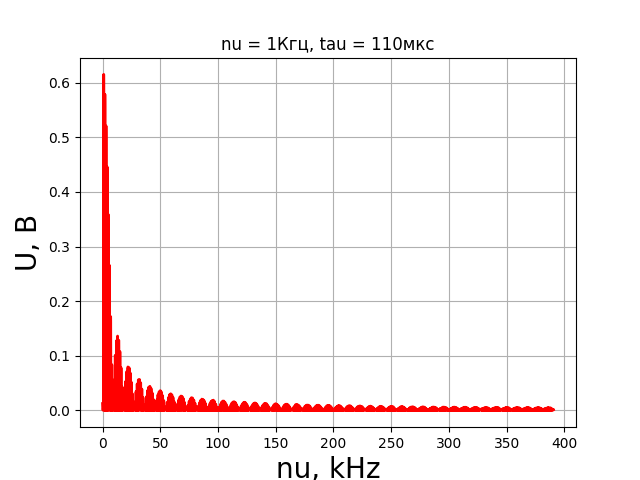
\includegraphics[width=\linewidth]{nu=1kHztau=110mks.png} 
    \caption*{$\tau$ = 110 мкс}
\end{minipage}

\caption{Заголовок вашей фигуры} % Основной заголовок для фигуры
\label{ris:experimentalcorrelationsignals}
\end{figure}

Как видно из графиков, при увеличении длительности сигнала уменьшается ширина спектра.

\item [\textbf{3.}] Измерим амплитуды $a_n$ и частоты $\nu_n$ спектральных гармоник при фиксированных $\nu_\text{повт}$ = 1кГц и $\tau$ = 50 мкс.

\begin{table}[!h]
\centering
\begin{tabular}{|l|l|l|l|l|l|l|}
\hline
$n$ гармоники & 1 & 2 & 3 & 4 & 5 & 6\\ \hline
$\nu_n^\text{эксп}$, кГц & 3.0 & 6.0 & 9.0 & 12.0 & 15.0 & 18.8 \\ \hline
$\nu_n^\text{теор}$, кГц & 3. & 6.0 & 9.0 & 12.0 & 15.0 & 18.0 \\ \hline
$|a_n|^\text{эксп}$, мВ & 791 & 699 & 607 & 414 & 240 & 174\\ \hline
$|a_n/a_1|_\text{эксп}$ & 1 & 0.884 & 0.767 & 0.523 & 0.303 & 0.220 \\ \hline
$|a_n/a_1|_\text{теор}$ & 1 & 0.891 & 0.725 & 0.524 & 0.312 & 0.114\\ \hline
\end{tabular}
\end{table}

Здесь $a_1$ = 143.8 мВ.
$$\nu_n^\text{теор} = \frac{n}{T}$$
$$|a_n|_\text{теор} = \frac{|\text{sin}\frac{\pi n \tau}{T}|}{\pi n}$$

\item[\textbf{4.}] Зафиксируем период повторения прямоугольного сигнала $T = 1 \text{мс}$, $\nu_\text{повт} = 1\text{кГц}$. Изменяя длительность импульса $\tau$ в диапазоне от
$\tau=T/50$ до $\tau=T/5$, измерим полную ширину спектра сигнала $\Delta \nu$ — от центра спектра ($\nu = 0$) до гармоники с нулевой амплитудой $a_n \approx 0$ и установим зависимость между $\Delta \nu$ и $\tau$, полученную из формулы \ref{eq5}.

\begin{table}[h!]
\centering
\begin{tabular}{|c|c|c|c|c|c|c|c|}
\hline
$\tau$, мкс & 20 & 40 & 60 & 80 & 100 & 120 & 140 \\ \hline
$\Delta \nu$, кГц & 50 & 25 & 17 & 12.5 & 10 & 7.5 & 5 \\ \hline
$1/\tau \cdot 10^3$, с$^{-1}$ & 50.0 & 25.0 & 16.7 & 12.5 & 10 & 8.3 & 7.1 \\ \hline
\end{tabular}
\caption{Исследование зависимости $\Delta \nu$ и $\tau$}
\label{table2}
\end{table}
Построим график $\Delta
u\left(\frac{1}{\tau}\right)$. Используя МНК, получим $k=1.0229\pm0,0223$, откуда с хорошей точностью можем заключить, что $\Delta
u\frac{1}{\tau}=1$, что экспериментально доказывает соотношение неопределённостей. График приведён на рис.12
\begin{figure}[H] % Изменение на [H]
\centering
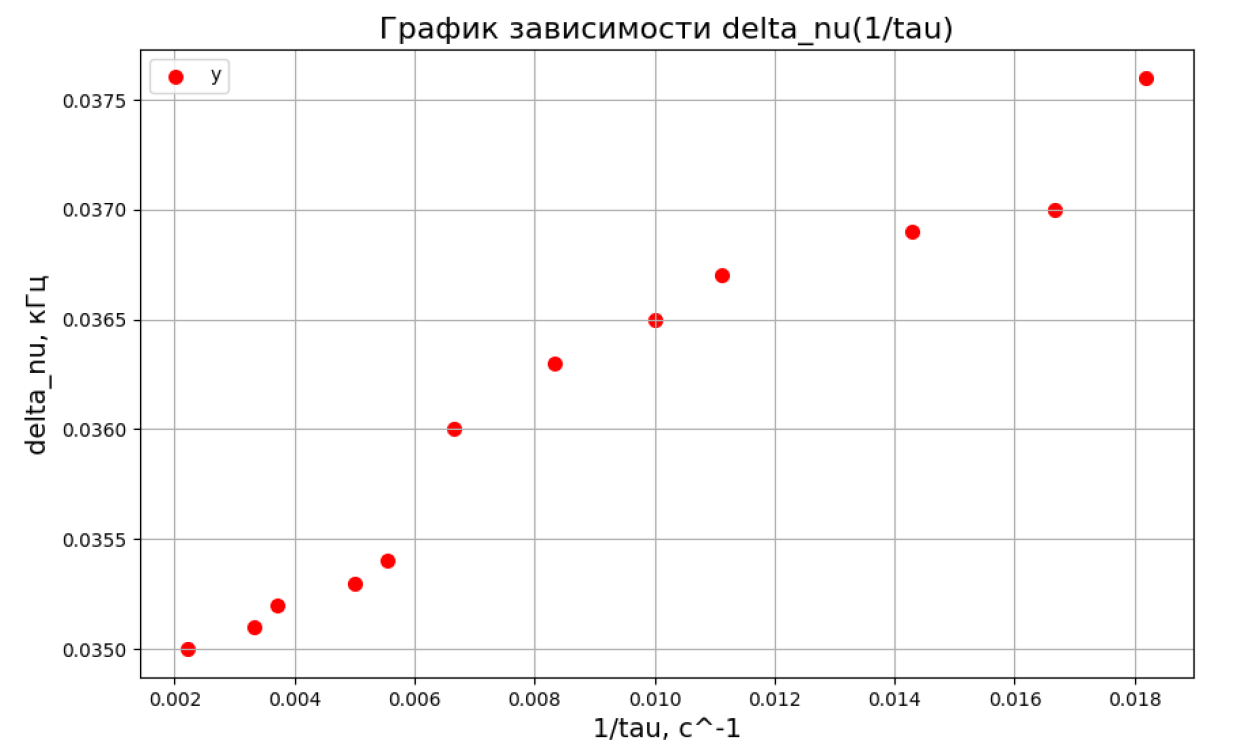
\includegraphics[width=0.7\linewidth]{Снимок экрана 2024-12-20 222205.png}
\caption{Зависимость $\Delta \nu$ от $1/\tau$}
\label{grafic1}
\end{figure}

\item[\textbf{5.}]
Зафиксируем длительность импульса прямоугольного сигнала $\tau = 100 \text{мкс}$. Изменяя период повторения $T$ в диапазоне от $2\tau$ до $50\tau$ измерим расстояния $\delta
u = \nu_{n+1} - \nu_n$ между соседними гармониками спектра.
\begin{table}[h!]
\centering
\begin{tabular}{|c|c|c|c|c|c|c|c|c|c|c|c|}
\hline
$T$, мкс & 200 & 500 & 1000 & 1500 & 2000 & 2500 & 3000 & 3500 & 4000 & 4500 & 5000 \\ \hline
$\delta \nu$, кГц & 5 & 2 & 1 & 0.688 & 0.459 & 0.400 & 0.330 & 0.287& 0.250 & 0.220& 0.200 \\ \hline
\end{tabular}
\caption{Зависимость $\delta \nu$ от $T$}
\label{table3}
\end{table}
\begin{figure}[H] % Изменение на [H]
\centering
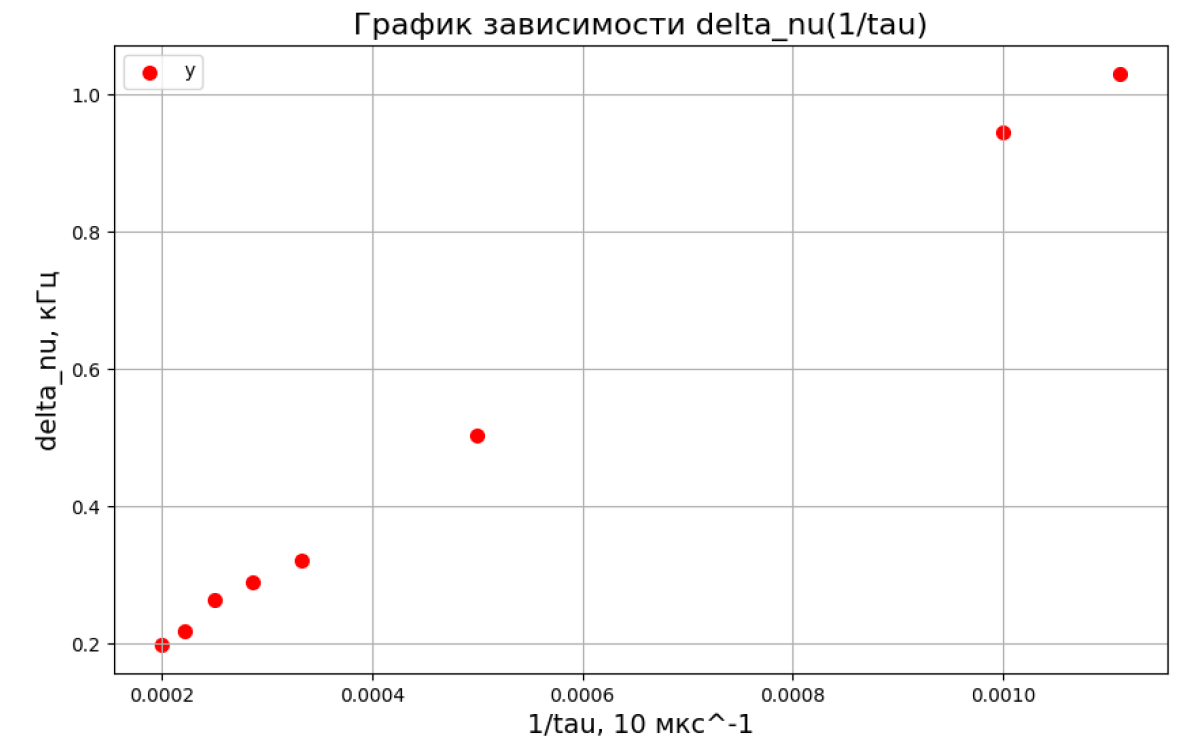
\includegraphics[width=0.7\linewidth]{Снимок экрана 2024-12-20 222153.png}
\caption{Зависимость $\delta \nu$ от $1/T$}
\label{grafic2}
\end{figure}
Построим график $\delta
u\left(\frac{1}{T}\right)$. Используя МНК, получим $k=1.001\pm0.003$, что экспериментально доказывает соотношение неопределённостей. График приведён на рис.13.
\end{enumerate}
\subsection*{Г. Наблюдение спектра амплитудно-модулированного сигнала}

\begin{enumerate}

\item [\textbf{1.}] Настраиваем генератор в режим модулированного по амплитуде синусоидального сигнала с несущей частотой $\nu_0$ = 50 кГц, частотой модуляции
$\tau_{RC}$

\begin{equation*}
K(1/\nu) = \frac{1}{2\pi \tau_{RC}} \left(\frac{1}{\nu}\right)
\end{equation*}

Построим график $K(1
u)$.

\begin{table}[h!]
\centering
\begin{tabular}{|c|c|c|c|c|c|c|}
\hline
$1/\num, \text{ кГц}^{-1}$ & 1.000 & 0.500 & 0.333 & 0.250 & 0.200 & 0.167 \\ \hline
$K_n$ & 0.380 & 0.190 & 0.120 & 0.071 & 0.078 & 0.042 \\ \hline
\end{tabular}
\caption{Отношение амплитуд спектральных гармоник фильтрованного и исходного сигналов}
\label{tab:RC}
\end{table}
\end{enumerate}

Из коэффициента наклона получаем

\begin{equation*}
\tau_{RC} = (3.3 \pm 0.2)мкс
\end{equation*}

\begin{figure}[H] % Изменение на [H]
\centering
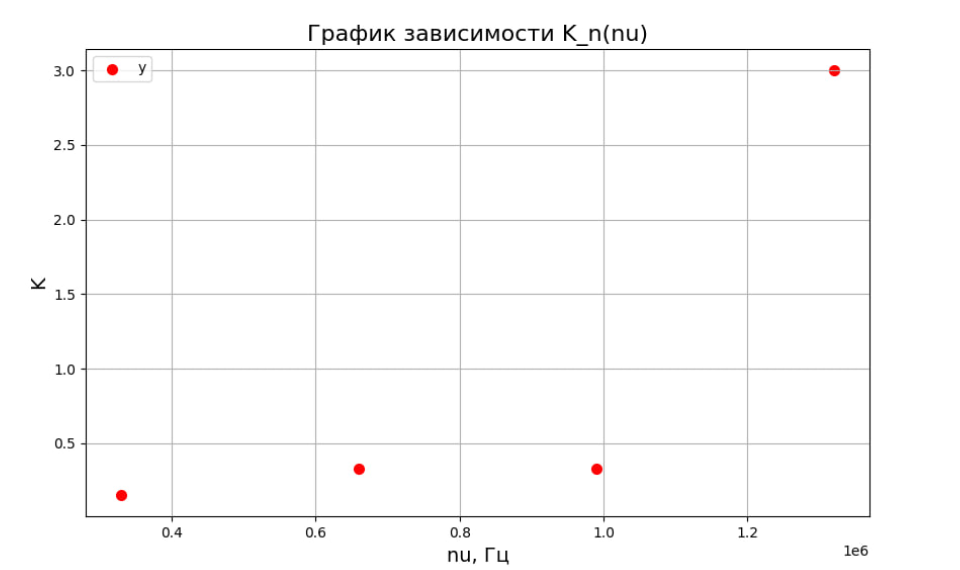
\includegraphics[width=15cm]{Снимок экрана 2024-12-21 005022.png}
\caption{Зависимость K от $\frac{1}{\nu}$}
\label{fig:RC}
\end{figure}
\section{Обсуждение результатов и выводы}

В данной работе мы изучили понятие спектра и спектрального анализа, исследовали спектральный состав периодических электрических сигналов, а также проанализировали фильтрацию сигналов при прохождении их через $RC$ контур. Проверили частный случай выполнения соотношения неопределённости.

\end{document}
